\section{Esempi di processi di Markov}
\label{sub:Lezione 5}
\mylocaltoc
\subsection{Processo di Wiener}%
\label{sub:Processo di Wiener}
Un processo di Wiener è modellato dall'equazione di Fokker-Plank così definita:
\begin{greenbox}{}
    \[
	\frac{\partial }{\partial t} P(\omega,t|\omega_0, t_0) =
	\frac{1}{2}\frac{\partial ^2}{\partial \omega^2} P(\omega, t|\omega_0, t_0) 
    .\] 
\end{greenbox}
\noindent
Questa corrisponde alla forma differenziale di Chapman-Kolmogorov in 1D con $A = 0$, $B = $const, $\Phi = 0$.\\
Inoltre si impone la seguente condizione iniziale:
\[
    P(\omega,t_0|\omega_0, t_0) = \delta (\omega-\omega_0) 
.\]
Il processo si può risolvere utilizzando la funzione caratteristica:
\[
    \phi (s, t) = \int d\omega P(\omega, t|\omega_0, t_0) e^{is\omega}
.\] 
Sfruttando le regole della trasformata possiamo riscrivere l'equazione del processo come:
\[
    \frac{\partial \phi }{\partial t} = -\frac{1}{2}s^2\phi
.\] 
\[
    \phi (s, t_0) = \exp (is\omega_0) 
.\] 
La soluzione è nota:
\[\begin{aligned}
    \phi (s) =& \exp\left(-\frac{1}{2}s^2\left(t-t_0\right)\right)\phi (s,t_0)  =\\
    	=&\exp\left(-\frac{1}{2}s^2\left(t-t_0\right) + is\omega_0 \right) 
.\end{aligned}\]
Visto che l'antitrasformata di una Gaussiana è una Gaussiana abbiamo la soluzione nello spazio reale:
\begin{redbox}{Soluzione del processo di Wiener}
    \[
	P(\omega,t|\omega_0, t_0) = 
	\frac{1}{\sqrt{2\pi\left(t-t_0\right)} }
	\exp\left(- \frac{\left(\omega-\omega_0\right)^2}{2\left(t-t_0\right)}\right)
    \] 
\end{redbox}
\noindent
Il processo che abbiamo ottenuto è Gaussiano:
\begin{align}
    &\left<\omega\right> =  \omega_0 \label{eq:mean_wiener}\\
    &\left<\left(\omega-\omega_0\right)^2\right> = t- t_0 \label{eq:var_wiener}
.\end{align}
\paragraph{Proprietà dei processi di Wiener}%
\label{par:Proprietà dei processi di Wiener}
\begin{itemize}
    \item \'E continuo.
    \item Non è differenziabile, $\forall k$:
	\[\begin{aligned}
	    \text{Prob}&\left(\frac{\left|\omega (t+h) - \omega (t) \right|}{h}> k\right) = \\
		       & = 2 \int_{kh}^{\infty} d\omega  \frac{1}{\sqrt{2\pi  h}} e^{- \omega^2 /2h} = \\
		       &=1-\mbox{erf}\left(k \sqrt{\frac{k}{2}} \right) = \\
		       &=1- \frac{2}{\sqrt{\pi} } \sum_{n=0}^{\infty} \frac{(-1)^n \left[k\sqrt{\frac{h}{2}} \right]^{2n + 1}}{n! (2n+1) }
		       \ \xrightarrow[]{h\to 0} 1
	.\end{aligned}\]
	Quindi $\forall k$ grande a piacere quando $h\to 0$ si ha che:
	\[
	    \frac{\omega (t + h)-\omega (t)}{h}>k
	.\] 
	Questo implica la non differenziabilità del processo.
    \item Gli incrementi sono indipendenti:
	\[\begin{aligned}
	    P(&\omega_2, t_2; w_1,t_1; \omega_0,t_0) = \\
	      &= P(\omega_2, t_2|\omega_1,t_1) P(\omega_1, t_1|\omega_0,t_0) P(\omega_0,t_0) 
	.\end{aligned}\]
	Il primo termine dopo l'uguale non dipende da $(\omega_0,t_0)$ perché il processo è Markoviano.
    \item La correlazione: \\
	Ipotizziamo di avere $t>s$:
	\[\begin{aligned}
	    \left<\omega (t) \omega (s)\right> &= \left<\left(\omega (t) -\omega (s)\right)\omega (s) \right>+\left<\omega^2(s) \right> =\\
					       &=\left<\left(\omega (t)-\omega (s)\right)\right>\left<\omega(s)\right> + s = s
	.\end{aligned}\]
    In cui nel primo passaggio si somma e si sottrae $\omega (s)$, nel secondo passaggio si ha che l'incremento $\omega (t)-\omega (s)$ è indipendente da $\omega (s)$, quindi la media del prodotto corrisponde al prodotto delle medie. Tuttavia l'incremento è distribuito come una gaussiana a media nulla, quindi il primo termine si annulla. Il secondo termine invece è pari a $s$ per l'equazione \ref{eq:var_wiener}.\\
    Nel caso generale si ha che:
    \[
        \left<\omega (t)\omega (s)| \left[\omega_0t_0\right]\right> = \min(t-t_0, s-t_0) + \omega_0^2
    .\] 
    Che nel caso particolare in cui $\omega_0=t_0=0$ si ricongiunge a quello visto sopra $\left<\omega (t) \omega (s) \right> = s$ se $t>s$.
    \usetikzlibrary{math}
    \tikzmath{\x = 5; \y = 4;}
    \begin{center}
    \begin{tikzpicture}
	 \draw[-stealth] (0,0) --(\x/\y, 0)node[below]{$s$} -- (\x,0) node[right]{$t$};
	 \draw[-stealth] (0,0) --(0,\x/\y)node[left]{$s$} -- (0,\x*2/5) node[above]{$\left<\omega (t) \omega (s) \right>$};
         \draw[thick] 
		  (0,0) node[below]{$0$} -- 
		  (\x/\y,\x/\y)  -- 
		  (\x,\x/\y);
	 \draw[dash dot] 
		  (\x/\y, 0) --
		  (\x/\y, \x/\y);
	\draw[dash dot] 
		  (0,\x/\y) --
		  (\x/\y, \x/\y);

    \end{tikzpicture}
    \end{center}
    \noindent
\end{itemize}

\subsection{Processo di Ornstein - Uhlenback}%
\label{sub:Processo di Ornstein - Uhlenback}
Prendiamo in considerazione altri esempi di processi di Markov.
\begin{redbox}{Equazione di Ornstein - Uhlenback}
    \[
	\frac{\partial P}{\partial t} = \frac{\partial }{\partial x} (kxP) + \frac{1}{2}D\frac{\partial ^2}{\partial x^2} P
    .\] 
\end{redbox}
\noindent
\subsubsection{Soluzione stazionaria}%
\label{subsub:Soluzione stazionaria}
Cerchiamo intanto la soluzione con ($\partial_{t}P=0$):
\[
    \frac{\partial }{\partial x} \left(kxP + \frac{1}{2}D \frac{\partial }{\partial x} P\right) = 0 \implies
\] 
\[
    \implies  \left[kxP + \frac{1}{2}D \frac{\partial }{\partial x} P\right]_{-\infty}^{x} = J
.\] 
Se ipotizziamo che:
\[\begin{aligned}
    & 1. \ \lim_{\left|x\right| \to \infty} P(x, t|x_0,t_0) = 0 \\
    & 2. \ \lim_{\left|x\right| \to \infty} xP(x, t|x_0,t_0) = 0
.\end{aligned}\]
Allora possiamo affermare che la corrente $J=0$ per $x\to \infty$. Si risolve allora l'equazione differenziale:
\begin{bluebox}{Soluzione stazionaria}
    \begin{equation}
	P_s(x) = \frac{1}{\sqrt{\pi} D /k}e^{-kx^2 / D} \label{eq:5_staz}
    \end{equation}
\end{bluebox}
\noindent
\subsubsection{Soluzione dipendente dal tempo.}%
\label{subsub:Soluzione dipendente dal tempo}
Per la dipendenza temporale sfruttiamo la funzione caratteristica $\phi (s)$.
\[
    \phi (s) = \int e^{isx}P(x,t|x_0,t_0) dx
.\] 
L'equazione del processo diventa:
\[
    \partial_{t}\phi  = -ks\partial_{s}\phi  - \frac{1}{2}Ds^2\phi
.\] 
Questa equazione alle derivate parziali può essere risolta tramite il metodo delle caratteristiche (\ref{sub:caratteristiche}).\\
L'unico ostacolo all'utilizzo del metodo è il secondo termine dopo l'uguale (contiene la soluzione), vorremmo ricondurci all'equazione in forma standard. \\
Facciamo allora il cambio di variabile:
\[
    g = \ln\phi 
.\] 
Visto che:
\[
     \partial_{t}g =\frac{\partial_{t}\phi}{\phi} \qquad 
     \partial_{s}g = \frac{\partial_{s}\phi}{\phi}
.\] 
Si ha una equazione in $g$ più maneggevole:
\[
    \partial_{t}g + k s \partial_{s}g = -\frac{1}{2}Ds^2
.\] 
Questa è risolubile con il metodo delle caratteristiche: 
\[
    (a, b, c) \to (1, ks, -\frac{1}{2}Ds^2) 
.\] 
Parametrizzando con $\eta$ abbiamo le equazioni caratteristiche:
\[
        \frac{\text{d} t}{\text{d} \eta} = 1 
	\qquad
	\frac{\text{d} s}{\text{d} \eta} = ks 
	\qquad
	\frac{\text{d} g}{\text{d} \eta} = -\frac{1}{2}D s^2
.\] 
Possiamo risolvere per rimuovere $\eta$:
\[
    \begin{cases}
        1. \quad dt = \dfrac{ds}{ks}\\
	2. \quad \dfrac{ds}{ks} = - \dfrac{dg}{1 / 2 Ds^2}
    \end{cases}
\] 
Integrando queste equazioni escono fuori delle costanti, ridefinendo tali costanti come funzioni ($u_1,u_2$) saremo in grado di risalire alla $\phi$.\\ 
Risolviamo la 1:
\[
    c_1 = t - \frac{1}{k}\ln (s) \ \implies  \ c'_1 = \exp\left(t- \frac{1}{k}\ln (s) \right) = s e^{-kt}
.\] 
Quindi definiamo la prima soluzione come $u_1$:
\begin{equation}
    u_1(t,s) = s e^{-kt} \label{eq:cat1}
\end{equation}
Passiamo alla equazione 2 del sistema, integrando si ottiene:
\[
    c_2 = \frac{s^2D}{4k} + g 
.\] 
Ricordando che $g=\ln\phi$ possiamo definire anche un'altra funzione a partire dalla costante $c_2$ (si fa l'esponenziale della 2):
\begin{equation}
    u_2(t,s) = \phi \exp\left(\frac{Ds^2}{4k}\right) \label{eq:cat2}
\end{equation}
Riscrivendo la \ref{eq:cat2} isolando $\phi$ si ha:
\[
    \phi  = u_2 \exp\left(-\frac{Ds^2}{4k}\right)
.\]
Visto che $u_1$ e $u_2$ sono entrambe costanti collegate dalle equazioni caratteristiche sarà vero che:
\[
    u_2 = f(u_1) 
.\] 
\begin{redbox}{Soluzione dipendente dal tempo per $\phi$}
    \begin{equation}
    \phi =f\left(se^{-kt}\right)\exp\left(-\frac{Ds^2}{4k}\right) 
    \label{eq:car_phi}
    \end{equation}
\end{redbox}
\noindent
\subsubsection{Condizioni al contorno}%
\label{subsub:Condizioni al contorno}
\[
    P(x,0|x_0,0) = \delta (x-x_0) \implies  \phi (s,0) = e^{ix_0s}
.\] 
Prendiamo l'equazione \ref{eq:car_phi} ed invertiamola per trovare la $f(s)$ ($t=0$) inserendo anche la condizione iniziale:
\[
	f(s) = e^{ix_0s}\exp\left(\frac{Ds^2}{4k}\right)
.\] 
Per reinserire il tempo e trovare la soluzione con queste condizioni iniziali basta fare la sostituzione:
\[
    s \to se^{-kt}
.\] 
\begin{redbox}{Soluzione con condizione iniziale $\delta$}
    \begin{equation}
	\phi(s,t) =
	\exp\left[-\frac{Ds^2}{4k}\left(1-e^{-2kt}\right) + isx_0e^{-kt}\right]
    \end{equation}
\end{redbox}
\noindent
A questo punto possiamo tornare indietro con una antitrasformata, altrimenti possiamo ricavare i momenti sfruttando le proprietà di $\phi$:
\[
    \left<x(t)\right> = \left.i\frac{\partial \phi}{\partial s} \right|_{s=0} = x_0e^{-kt}
.\] 
\[\begin{aligned}
    \text{var(x(t) )} =& \left<x^2(t)\right> - \left<x(t)\right>^2 = \\
    =& \left.-1 \frac{\partial ^2\phi}{\partial s^2}\right|_{s=0} - \left<x\right>^2 = \\
    =&\frac{D}{2k}\left(1-e^{-2kt}\right)
.\end{aligned}\]

\begin{figure}[H]
    \centering
    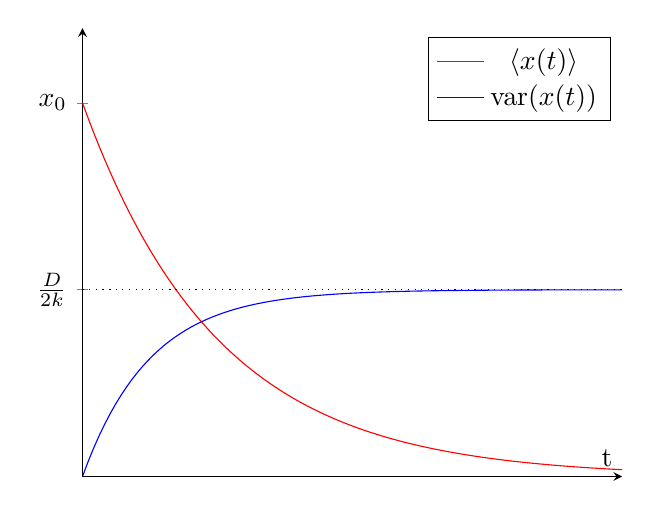
\begin{tikzpicture}
	\begin{axis}[
	    xmin= 0, xmax= 4,
	    ymin= 0, ymax = 1.2,
	    axis lines = middle,
	    xlabel={t},
	    ylabel={},
	    ytick={0.5, 1},
	    yticklabels={$\frac{D}{2k}$, $x_0$ },
	    xtick={0},
	    xticklabel={$$},
	]
	\addplot[domain=0:4, samples=100, color=red]{e^(-x)};
	\addlegendentry{$\left<x(t) \right>$ }
	\addplot[domain=0:4, samples=100, color=blue]{1/2*(1-e^(-2*x) ) };
	\addlegendentry{var($x(t)$) }
	\addplot[dotted, domain=0:4, samples=100]{0.5};
	\end{axis}
    \end{tikzpicture}
    \caption{\scriptsize Andamento della media e della varianza per il processo di Ornstein-Uhlenback.}
    \label{fig:mean-var}
\end{figure}
\noindent
I risultati ottenuti sono conformi con le condizioni iniziali inserite. 
\paragraph{Media}%
all'istante iniziale tutti i camminatori sono in $x_0$ (grazie alla $\delta$). \\
Quando il processo fa evolvere le posizioni dei camminatori allora i camminatori si allontanano da $x_0$ andando verso l'origine, questo è conforme con quanto visto per la soluzione stazionaria: una Gaussiana centrata nello $0$.
\paragraph{Varianza}%
Nell'istante iniziale, quando tutti i camminatori sono nel punto $x_0$, la varianza è nulla, questa si stabilizza nel tempo al valore dato dalla Gaussiana nelle condizioni stazionarie.
\subsubsection{Calcolo delle correlazioni}%
\label{subsub:Calcolo delle correlazioni}
\[\begin{aligned}
    \left<x(t_1) x(t_2) \right.&\left.|\left[x_0,t_0\right]\right> =\\
    =&\int dx_1dx_2 P(x_1,t_1;x_2,t_2;x_0,t_0) x_1x_2 = \\
    =&\int dx_1dx_2 x_1x_2P(\overline{x}_1,\overline{x}_2) P(\overline{x}_2, \overline{x}_0) 
.\end{aligned}\]
In cui si è assunto il processo Markoviano e la gerarchia temporale: $t_1>t_2>t_0$.\\
Se il processo ha raggiunto la stazionarietà ($t_0\to \infty$) allora conosciamo la forma del propagatore:
\[
    P(x_2|x_0) \sim \exp\left(-k \frac{x_2^2}{D}\right)
.\] 
Risolvendo con questa si ottiene:
\begin{redbox}{Correlazione temporale a due}
    \[
	\left<x(t) x(s) \right> \sim \frac{D}{2k}\exp\left(-k\left|t-s\right|\right)
    .\] 
    La correlazione temporale delle posizioni decade esponenzialmente.
\end{redbox}
\noindent

\subsubsection{Ornstein-Uhlenback come modello per rumore realistico.}%
\label{subsub:Ornstein-Uhlenback come modello per rumore realistico.}
Facendo la trasformata di Fourier della funzione di Correlazione si ottiene una Lorenziana:
\[\begin{aligned}
    S_{OU}(\omega) = & \mathcal{F}\left(\left<x(t) x(s) \right>\right)=\\
		     =&\frac{1}{\omega^2 /k ^2 + 1}
.\end{aligned}\]

\begin{figure}[H]
    \centering
    \begin{tikzpicture}
	\begin{axis}[
	    xmin= 0, xmax= 4,
	    ymin= 0, ymax = 1.5,
	    axis lines = middle,
	    xlabel={$\omega$},
	    ylabel={$S_{OU}(\omega)$},
	    ytick={1, 0.5},
	    yticklabels={$S_{OU}(0)$, $S_{OU}(0)/2$ },
	    xtick={0, 1},
	    xticklabels={$$ ,$\sim k$},
	    every axis x label/.style={
		at={(axis description cs:1,-0.1)},
		anchor=south,
                },
	]
	\addplot[domain=0:4, samples=100, color=red]{1/(x^2 + 1) };
	\addplot[dotted, domain=0:1, samples=100]{0.5};
	\addplot[dotted, domain=0:1, samples=100] coordinates{(1,0)(1,0.5)};
	\end{axis}
    \end{tikzpicture}
    \caption{\scriptsize Andamento della trasformata della correlazione per il processo di Ornstein-Uhlenback.}
    \label{fig:mean-var}
\end{figure}
\noindent
Questo è esattamente quello che ci aspettiamo da un rumore realistico: il rumore ha una frequenza di cut-off dettata da una Lorenziana.	\\
Il cut-off è dovuto al fatto che le cose non possono muoversi infinitamente veloci, l'inerzia dei corpi che partecipano al moto stocastico fissa la frequenza di cut-off.\\
C'è quindi un tempo caratteristico di osservazione del fenomeno
\[
    \tau  = \frac{1}{k}
.\] 
Se osserviamo il moto su scale temporali di quest'ordine allora lo spettro degli urti tra i corpi va a zero, questo comporta che il moto oltre queste scale temporali non è più ben descritto dal processo di Wiener.
\begin{ex}{Modifica all'equazione di OU}
    Risolvere l'equazione di Ornstein-Uhlenback con l'aggiunta di un termine nella $\partial_{x}$:
    \[
	\frac{\partial P}{\partial t} = \frac{\partial }{\partial x} (\left(kx + \alpha\right)P) + \frac{1}{2}D\frac{\partial ^2}{\partial x^2} P
    .\] 
    \textbf{Soluzione}: Il moto dovrebbe andare a stazionarietà nel punto $-\alpha  / k$.
\end{ex}
% Appendice
%%%%%%%%%%%%%%%%%%%%%%%%%%
%  Codice per appendice  %
%%%%%%%%%%%%%%%%%%%%%%%%%%
\noindent\rule{0.48\textwidth}{0.7pt}
\newpage
\addtocounter{Sec}{\value{section}}%Mantengo il numero delle sezioni
\begin{appendices}
\section*{Appendice}%
\setcounter{section}{\theSec}%Applico numero sezioni
\setcounter{subsection}{0}%Applico numero sezioni
\renewcommand{\thesubsection}{\arabic{section}.\Alph{subsection}}

\subsection{Metodo delle Caratteristiche.}
\label{sub:caratteristiche}
Supponiamo di avere una PDE della forma:
\begin{redbox}{PDE per metodo delle caratteristiche}
\[
    a(x,y) \partial_{x}u + b(x,y) \partial_{y}u - c(x, y) = 0
.\] 
\end{redbox}
\noindent
Scrivibile anche come:
\begin{equation}
    \left(a,\ b,\ c\right)\cdot \left(\partial_{x}u,\ \partial_{y}u,\ -1\right) = 0
    \label{eq:caratt}
\end{equation}
Ed una superficie parametrizzata con la soluzione della PDE ($u(x,y))$: 
\[
    S \equiv (x,y, u(x,y) ) 
.\] 
%\begin{center}
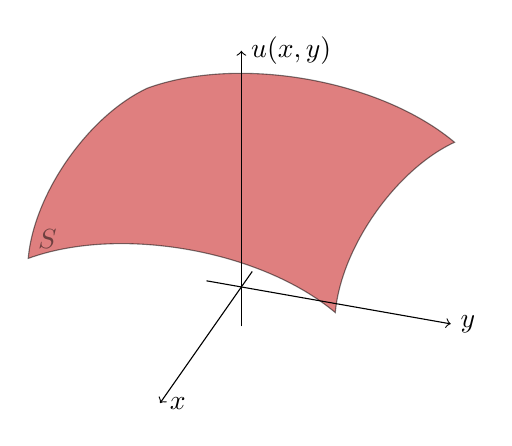
\begin{tikzpicture}[x={(170:.9cm)},y={(55:.6cm)},z={(90:1cm)}]
  %%%%%%%%%%%%%%%%%%%%
  %  Piano Tangente  %
  %%%%%%%%%%%%%%%%%%%%
  \tikzmath{\x = 2.2; \z = -0.4;}
  %%%%%%%%%%%%%%%%%
  %  Piano curvo  %
  %%%%%%%%%%%%%%%%%
  \draw[fill=red!75!black, opacity=0.5, looseness=.8] (\x,-\x,\z) node[above right] {$S$}
  to[bend left] (\x,\x,\z)
  to[bend left] coordinate (mp) (-\x,\x,\z)
  to[bend right] (-\x,-\x,\z)
  to[bend right] coordinate (mm) (\x,-\x,\z)
  -- cycle;
  %%%%%%%%%%
  %  Assi  %
  %%%%%%%%%%
  \draw[->] (0.5,0,-1.5) -- (-3,0,-1.5) node[right] {$y$};
  \draw[->] (0,0.4,-1.5) -- (0,-3,-1.5) node[right] {$x$};
  \draw[->] (0,0,-2) -- (0,0,1.5) node[right] {$u(x,y)$};
\end{tikzpicture}
\end{center}

\noindent
\subsubsection{Vettore tangente a $S$}%
\label{subsub:Vettore tangente a S}
\begin{bluebox}{}
Il vettore $\left(a, \ b, \ c\right)$ appartiene al piano tangente di $S$ in ogni punto $\left(x, y, z\right)$.
\end{bluebox}
\noindent
La normale $\vect{N}$ alla superficie $S$ la si trova facendo il gradiente di:
\[
    \overline{S} = u(x,y) - z
.\] 
Si ottiene quindi:
\[
    \vect{N}  = \left(\partial_{x}u, \ \partial_{y}u, \ -1\right)
.\] 
Visto che $\vect{N}$ è il secondo termine nella \ref{eq:caratt} si vede che la soluzione è il luogo dei vettori $(a, b,c)$ ortogonali a $\vect{N}$, quindi tangenti al piano $S$.
%\begin{center}
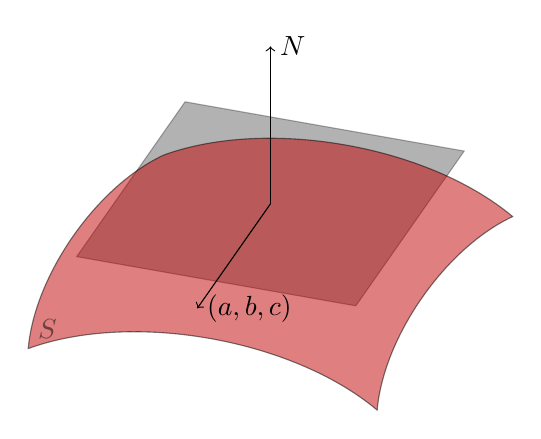
\begin{tikzpicture}[x={(170:.9cm)},y={(55:.6cm)},z={(90:1cm)}]
  %%%%%%%%%%%%%%%%%%%%
  %  Piano Tangente  %
  %%%%%%%%%%%%%%%%%%%%
  \tikzmath{\x = 2.; \z = 0;}
  \draw[fill=black, opacity=0.3] (\x,-\x,\z) -- (\x,\x,\z) -- (-\x,\x,-\z) -- (-\x,-\x,-\z) -- cycle;
  %%%%%%%%%%%%%%%%%
  %  Piano curvo  %
  %%%%%%%%%%%%%%%%%
  \draw[fill=red!75!black, opacity=0.5, looseness=.8] (2.5,-2.5,-1) node[above right] {$S$}
  to[bend left] (2.5,2.5,-1)
  to[bend left] coordinate (mp) (-2.5,2.5,-1)
  to[bend right] (-2.5,-2.5,-1)
  to[bend right] coordinate (mm) (2.5,-2.5,-1)
  -- cycle;
  %%%%%%%%%%
  %  Assi  %
  %%%%%%%%%%
  \draw[->] (0,0,0) -- (0,-2.7,0) node[right] {$(a, b, c) $};
  \draw[->] (0,0,0) -- (0,0,2) node[right] {$N$};
\end{tikzpicture}
\end{center}

\noindent
Quindi la soluzione della PDE è tale per cui il vettore $(a,b,c)$ sta sul piano tangente.

\subsubsection{Curva caratteristica}%
\label{subsub:Curva caratteristica}
Per mappare la soluzione si introduce una curva $C$ detta curva caratteristica che descrive la superficie. 
\[
    C: \quad C \equiv \left(x(\eta) , y(\eta), z(\eta) \right)
.\] 
$C$ è una curva parametrica in $\eta$ localmente tangente a $(a, b, c)$.\\
La condizione di parallelismo implica il seguente sistema:
\begin{greenbox}{Equazioni Caratteristiche}
    Sono curve integrali per il campo vettoriale $(a, b, c)$ 
\[
    \begin{cases}
	 &a(x(\eta) , y(\eta) ) = \dfrac{\text{d} x}{\text{d} \eta} \\
								   &\\
	 &b(x(\eta) , y(\eta) ) = \dfrac{\text{d} y}{\text{d} \eta} \\ 
								   &\\
	 &c(x(\eta) , y(\eta) ) = \dfrac{\text{d} z}{\text{d} \eta}  
    \end{cases}
\]
\end{greenbox}
\noindent
Queste equazioni risolvono la PDE.
\begin{exmp}[Equazione del trasporto.]
   \[
       u_t + a \cdot u_x = 0
   .\]  
   In questo caso si ha $(a, b, c) \to (a, 1, 0)$, quindi:
   \[\begin{aligned}
	   &\dfrac{\text{d} x}{\text{d} \eta} = a & \quad
	   &\dfrac{\text{d} t}{\text{d} \eta} = 1 & \quad
	   &\dfrac{\text{d} z}{\text{d} \eta} = 0 &
   \end{aligned}\]
   Passiamo alla risoluzione:
   \[
       \begin{cases}
	    x(\eta) = a\eta +c_1\\
	    t(\eta) = c_2 + \eta\\
	    z(\eta) = c_3
       \end{cases}
       \implies\quad
       \begin{cases}
           x -at = x_0\\
	   z=k
       \end{cases}
   \] 
   In cui si è effettuata dell'algebra per eliminare $\eta$ nel primo sistema. 
   \begin{itemize}
       \item La funzione che risolve il sistema di destra è la soluzione dell'equazione del trasporto. 
       \item  Graficamente le funzioni che risolvono sono delle rette con $z$ costante, l'unione di queste rette rappresenta $S$.
       \item Abbiamo ottenuto un fascio di soluzioni poiché non abbiamo imposto alcuna soluzione al contorno.
   \end{itemize}
   In conclusione $z$ dovrà essere funzione di $x-at$, quindi la soluzione generale sarà una funzione del tipo:
   \[
       z(x, t ) = f(x-at) \equiv u(x, t) 
   .\] 
   Supponiamo che all'istante iniziale la soluzione fosse una gaussiana:
   \[
       f(x, t=0) = e^{-x^2}
   .\] 
   Quindi si ha che anche la soluzione a $t=0$ è una gaussiana:
   \[
       u(x, t=0) = e^{-x^2}
   .\] 
   Ed introducendo il tempo la soluzione diventa semplicemente:
   \[
       u(x, t) = e^{-\left(x-at\right)^2}
   .\] 
   
\end{exmp}
\noindent

\end{appendices}

\renewcommand{\thesubsection}{\arabic{section}.\arabic{subsection}}
%%%%%%%%%%%%%%%%%%%%%%%%%


